\documentclass[border=10pt]{standalone}
\usepackage{tikz}

\usepackage{amssymb} %maths
\usepackage{amsmath} %maths
\usepackage[utf8]{inputenc} %utile pour taper directement les caractères accentués

\begin{document}

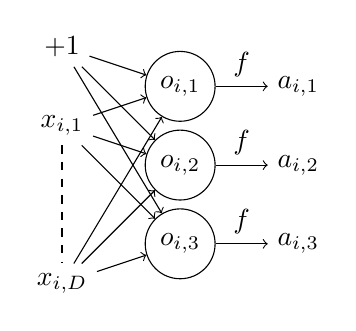
\begin{tikzpicture}
    \node[draw, circle] (oi1) at  (1.5,2.5) {$o_{i,1}$};
    \node[draw, circle] (oi2) at  (1.5,1.5) {$o_{i,2}$};
    \node[draw, circle] (oi3) at  (1.5,0.5) {$o_{i,3}$};

    \node (offset) at  (0,3) {$+1$};
    \node (xi1) at  (0,2) {$x_{i, 1}$};
    \node (xid) at  (0,0) {$x_{i, D}$};
    \node (ai1) at  (3,2.5) {$a_{i,1}$};
    \node (ai2) at  (3,1.5) {$a_{i,2}$};
    \node (ai3) at  (3,0.5) {$a_{i,3}$};

    \draw[->] (offset) -- (oi1) node[midway,above]{}; %$\beta_0$};
    \draw[->] (xi1) -- (oi1) node[midway,below]{}; %$\beta_1$};
    \draw[->] (xid) -- (oi1) node[midway,below]{}; %$\beta_D$};

    \draw[->] (offset) -- (oi2) node[midway,above]{}; %$\beta_0$};
    \draw[->] (xi1) -- (oi2) node[midway,below]{}; %$\beta_1$};
    \draw[->] (xid) -- (oi2) node[midway,below]{}; %$\beta_D$};

    \draw[->] (offset) -- (oi3) node[midway,above]{}; %$\beta_0$};
    \draw[->] (xi1) -- (oi3) node[midway,below]{}; %$\beta_1$};
    \draw[->] (xid) -- (oi3) node[midway,below]{}; %$\beta_D$};

    \draw[->] (oi1) -- (ai1) node[midway,above]{$f$};
    \draw[->] (oi2) -- (ai2) node[midway,above]{$f$};
    \draw[->] (oi3) -- (ai3) node[midway,above]{$f$};
    \draw[dashed] (xi1) -- (xid);
\end{tikzpicture}

\end{document}
